\item \points{15} {\bf Logistic Regression: Training stability}

In this problem, we will be delving deeper into the workings of logistic
regression. The goal of this problem is to help you develop your skills
debugging machine learning algorithms (which can be very different from
debugging software in general).

We have provided an implementation of logistic regression in
\texttt{src/stability/stability.py}, and two labeled datasets $A$ and $B$ in
\texttt{src/stability/ds1\_a.csv} and \texttt{src/stability/ds1\_b.csv}.

Please do not modify the code for the logistic regression training algorithm
for this problem. First, run the given logistic regression code to train two
different models on $A$ and $B$. You can run the code by simply executing
\texttt{python stability.py} in the \texttt{src/stability} directory.

\begin{enumerate}

  \item \subquestionpoints{2}
What is the most notable difference in training the logistic regression model
on datasets $A$ and $B$?


\ifnum\solutions=1 {
  \begin{answer}
\\ \\ 
The notable is that for Dataset A it converges at 30374 iteration whereas for Dataset B it never tends to converge at all Even after 1M iterations.
\\ \\
\end{answer}

} \fi

  \item \subquestionpoints{5}
Investigate why the training procedure behaves unexpectedly on dataset $B$, but
not on $A$. Provide hard evidence (in the form of math, code, plots, etc.) to
corroborate your hypothesis for the misbehavior. Remember, you should address
why your explanation does \emph{not} apply to $A$.

\textbf{Hint}: The issue is not a numerical rounding or over/underflow error.


\ifnum\solutions=1 {
  \begin{answer}
\begin{figure}[h!]
\centering
\begin{subfigure}{.5\textwidth}
  \centering
  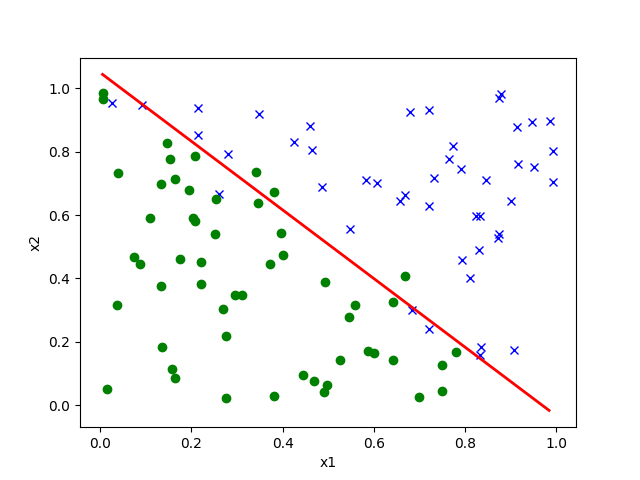
\includegraphics[width=.75\linewidth]{stability/0.png}
  \caption{Data A}
  \label{fig:sub1}
\end{subfigure}%
\begin{subfigure}{.5\textwidth}
  \centering
  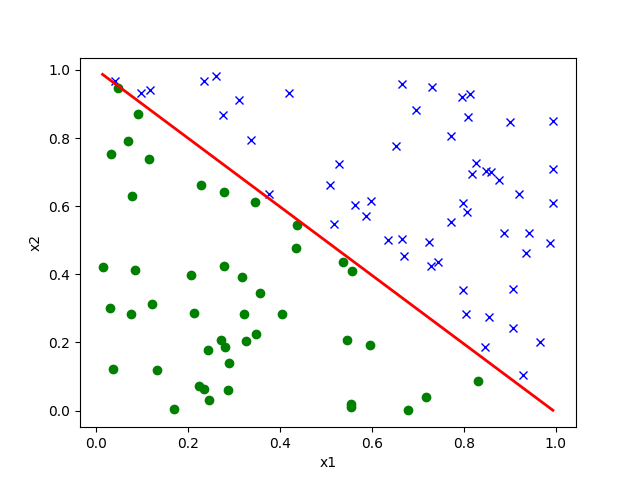
\includegraphics[width=.75\linewidth]{stability/1.png}
  \caption{Data B}
  \label{fig:sub2}
\end{subfigure}
\caption{Data B is perfectly seprable}
\label{fig:test}
\end{figure}

The reason is that dataset B is perfectly separable while A is not. LR without Regularisation as in the code will not converge to a single parameter because of the fact that it is perfectly separable. Since it is perfectly separable any $\theta$ \ that separates can decrease the loss but no change in boundary.
\\ \\

\end{answer}

} \fi


  \item \subquestionpoints{5}
For each of these possible modifications, state whether or not it would lead to
the provided training algorithm converging on datasets such as $B$. Justify your
answers.
\begin{enumerate}
  \item Using a different constant learning rate.
  \item Decreasing the learning rate over time (e.g. scaling the initial
  learning rate by $1/t^2$, where $t$ is the number of gradient descent
  iterations thus far).
  \item Linear scaling of the input features.
  \item Adding a regularization term $\|\theta\|_2^2$ to the loss function.
  \item Adding zero-mean Gaussian noise to the training data or labels.
\end{enumerate}
 


\ifnum\solutions=1 {
  \begin{answer}
\\ \\
\ i. No, Because the learning rate will just jump not converge without regularisation \\ \\
\ ii. No, Updates will become arbitrarily small after a while. \\ \\
iii. No, This will not affect the separability of Data \\ \\
\ iv. Yes, this will penalize large  norm of $\theta$ \ and make data to converge \\ \\
\ \ v. No maybe it will make data totally linearly inseparable \\ \\
\end{answer}

} \fi


  \item \subquestionpoints{3} Are support vector machines vulnerable to datasets like $B$? Why or why not? Give an informal
justification.



\ifnum\solutions=1 {
  \begin{answer}
\\ \\
SVMs are not vulnerable. Because of the fact that weight vector are normalised so this instability of LR is solved with SVMs.
\\ \\
\end{answer}

} \fi

\end{enumerate}
